\chapter{Dynamics of infectious agents}

\section{Infectious pattern}

\begin{figure}[h]
  \centering
  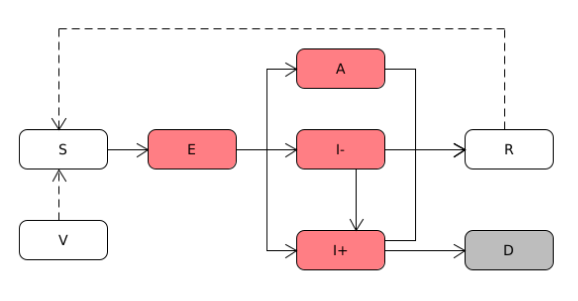
\includegraphics[width=\linewidth]{media/schema_infection.png}
  \caption{\centering {\small An overview of infectious pattern.}}
  \label{fig:schemainfection}
\end{figure}

\begin{tabular}{cc}
\parbox{0.5\linewidth}{S : Susceptible\\
A : Heals\\
D : Deceased\\
V : Vaccinated\\}
&
\parbox{0.5\linewidth}{E : Incubation phase\\
A : Asymptomatic patient\\
I- : Standard patient\\
I+ : Seriously ill\\}
\end{tabular}

\bigskip

Following the reflections of epidemiologists, we can break down the infectious  states of individuals as described above on the diagram. The continuous arrows represent a certain evolution that depends on several temporal and/or stochastic parameters. Those in dotted lines are more anecdotal. The phases in red correspond to the phase where the individual is a carrier and can transmit the infectious agent. The starting point of the population is in the susceptible state.\\

At the initialization of the infectious agent in the environment, according to a ratio and / or a certain initial amount, individuals are placed in the incubation phase. This selection is carried out randomly on all individuals in the environment. It may be interesting to determine more precisely the first individuals carriers and to study the difference in the spread of infectious agents. This is one of the interesting points of this project.\\

Each individual is in a specific state for each of the infectious agents in the environment. Competition between these agents can have an impact on their spread. For simplicity, when an individual is a carrier of an infection, he becomes ``immune'' to all other infections in the environment : he is then in one of three states among susceptible, cured or vaccinated according to his situation and experience.\\

\newpage

\section{State transitions}

\subsection{Susceptible}

Each infection is characterized by a contamination threshold that corresponds to the number of particles from which an individual enters the incubation phase. It seems wise to adapt it according to the age of the individual to represent the resistance of the organism. In a simplistic version, it is assumed that the number of particles emitted by a carrier individual is identical regardless of the infection, the infectious state of the carrier individual or the duration for which the individual has been a carrier. This design may be revised in a later version to add a factor in the particle emission based on the infectious score of the carrier individual. Two other parameters characterize the contamination of an infection :\\

\begin{itemize}

\item The time that a particle can persist in a place ; we will set this duration even if we can question a Gaussian approach. It was preferred to play on the efficiency of the persistent particles in places with the factor concerning the surface of place in the infectious evaluation.\\

\item The number of days that a particle can be accumulated in an individual ; this setting can hide another. We could take up the principle of an immediate reaction of the organism : the individual would constantly accumulate external particles, without defining a limited duration, and would produce an immune reaction. It will then be necessary to define an insufficient immune capacity to prevent the total particle from exceeding the contamination threshold. It should be noted that this new approach is inspired by the results obtained during this internship: individuals seem to become infected much too quickly without leaving a certain elasticity.\\

\end{itemize}

\subsection{Incubation phase}

When the individual is in the incubation phase, during which no symptoms are visible, two parameters characterize the infection : the mean and the standard deviation of the duration of incubation, which is assumed to follow a normal distribution, regardless of the characteristics of the individual. At the end of this random duration, the infectious status of an individual changes to one of three states : asymptomatic, standard or severe. This transition depends on the age of the individual and the infection.\\

When the incubation period is up, each individual is given a new infection score, such as an amount of infectious antigens in the body. This random score follows a normal distribution according to a mean and standard deviation characteristic of the infection. The idea is to define the infectious state of the individual according to this random amount. Indeed, it is possible to select two thresholds around which we can find three known probabilities in a Gaussian law. This distribution is also to be qualified according to the age of the individuals. Initially, the infectious representation of individuals is therefore described by a single score, assigned using a normal distribution with fixed parameters and regardless of the age of the individuals. The variation in infectious severity is therefore modeled by Gaussian bounds (a,b) that vary according to the age of the individuals. However, it seems more than wise to study the opposite degree of freedom for simplicity in a later version.\\

\begin{figure}[h]
  \centering
  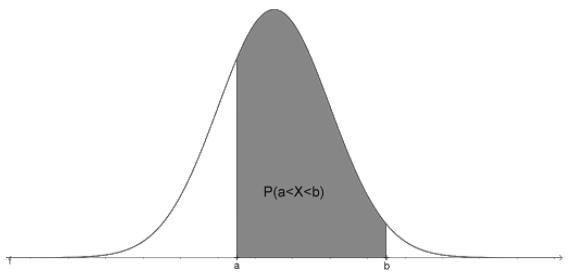
\includegraphics[width=0.5\linewidth]{media/loi_gauss.png}
  \caption{\centering {\small An overview of a Gaussian distribution.}}
  \label{fig:loigauss}
\end{figure}

\bigskip

Once the infectious score is initialized, the evolution of the infection is done by increasing or decreasing this score, according to parameters specific to the infectious status. In a natural way, the organism already tends to evolve on its own. If the infectious score becomes zero, the individual is cured, otherwise, if it exceeds a certain mortality threshold, the individual has died. To draw a parallel with a very simplistic medical view, this score can represent the difference between the number of antigens and antibodies of the individual.\\

\subsection{Asymptomatic patient}

\begin{wrapfigure}{l}{0.3\linewidth}
  \centering
  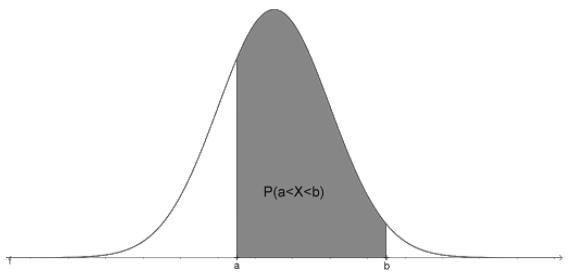
\includegraphics[trim = 0 0 334 0, clip, width=\linewidth]{media/loi_gauss.png}
\end{wrapfigure}

Each individual can heal on their own according to a certain daily self-healing score, much like an antibody production. For a first version, it is assumed that this score is a fixed amount and independent of the age of the individual. In view of the curve of the infectious score, this means that the healing time does not follow a normal distribution but rather a remission distribution that can be described as late. The healing score can therefore be revised in a later version depending on the observed data and the first results of the conception. It is assumed for simplicity that asymptomatic individuals are not susceptible to infectious care or aggravation.\\

When he is not aware of his asymptomatic infection, there is no change in behavior on the part of the individual ; this state does not cause infectious reflexes. Obviously, if his infection is identified, the individual will have to change his daily life to limit the epidemic spread according to territorial decisions. In a simple version, we are not interested in the propensity of the asymptomatic sick individual to adopt by himself a protective behavior in relation to the population by modifying his mobility. This means that only political decisions influence this state.\\

\subsection{Standard Sick}

\begin{wrapfigure}{l}{0.25\linewidth}
  \centering
  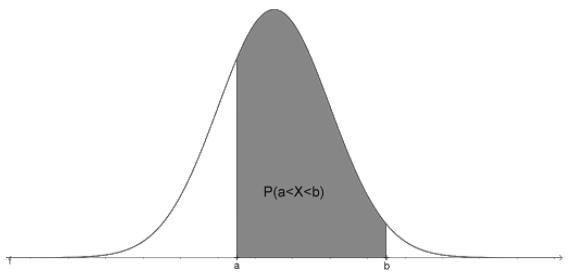
\includegraphics[trim = 234 0 184 0, clip, width=\linewidth]{media/loi_gauss.png}
\end{wrapfigure}

The standard infectious journey of an individual follows the same principle of self-healing as the asymptomatic one, except that it is possible/recommended for the individual to follow care. Whether through medical visits or medication, the individual's infectious score can be further reduced. Conversely, it is possible to undergo events that increase the individual's infectious score and eventually move it to the severe stage. Examples include poor care that is involuntarily perceived by the individual as nosocomial diseases or poor self-medication. Each type of care could be either positive or negative depending on a probability. These types of care would also be parameters to be implemented in each infection.\\

An individual in a state of standard infection has symptoms of infection and his daily life will be impacted by infectious reflexes. These infectious reflexes can push the individual to test himself or to introduce care into his daily life, whether medical visits or medication. Because of its weakened body, it will also tend to limit unnecessary travel. However, it is interesting to note that the symptoms do not necessarily reflect the identification of the infection : the individual will have to follow the policy regarding standard individuals only when it is evaluated by a doctor or an infectious test. Depending on territorial decisions, the daily lives of these individuals are also modified with constraints or obligations. These decisions may guide the individual to identify his condition.\\

\subsection{Seriously ill}

\begin{wrapfigure}{l}{0.25\linewidth}
  \centering
  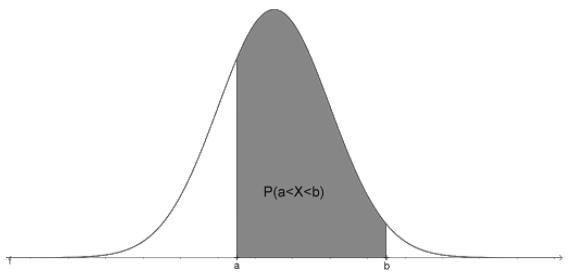
\includegraphics[trim = 384 0 0 0, clip, width=\linewidth]{media/loi_gauss.png}
\end{wrapfigure}

Individuals in a serious infectious state resume the same principle of care as standard patients. The care would then be different. In addition, no self-curing is performed by the individual and the infectious score increases daily. In practice, it is considered that its production of antibodies is not sufficient compared to that of antigens. This restricts design to simple antigen production, even if it deviates a little from a realistic medical model. The difference between this infectious worsening and the care available characterizes in a way the mortality of each infection. The individual is pushed for his survival to treat himself quickly : beyond a new threshold, the individual has died. An individual in a seriously ill condition does not need to be identified to be known : there is no distinction between the actual and known condition.\\

The infectious reflexes of these individuals become the daily priority of these people. Their survival instincts are not subject to territorial politics. Moreover, this policy must take into account the limited care resources of the territory to avoid abandoning its individuals in serious condition.\\

\subsection{Cured \& Vaccinated}

For a first conception, we will not be interested in reinfections after recovery or after vaccination of individuals. An individual in a vaccinated state does not need to be identified to be known : there is no distinction between actual and known status. The question arises, however, for the state cures. In a simplistic version, it is considered that when the real carrier state is over, the individual passes into a real and known healing state. It is simply a pragmatic issue. In digitalization, leaving a preservation time, which can be compared to a quarantine time, has very little impact on the study of epidemic spread. The question may arise more on the economic criterion. And it is not interesting to reason about a political decision in this sense in an initial conception.\\

\subsection{Deceased}

A deceased individual does not need to be identified to be known... In this infectious design, the deaths of individuals do not follow a mortality rate predefined by a data observed in reality. The mortality of individuals depends on the proportion of seriously ill individuals, the gap between the infectious worsening and the available care of the infection, and also on the success of individuals in ``surviving'' with this available care. It is not easy to directly match a mortality rate observed in reality with digitalization. This is probably one of the most delicate points of the infectious design : the mortality of an infection depends significantly on the dynamics of sick individuals. As a result, the realistic development of the mortality of the infection needs to be deepened.\\

\newpage

\section{Care, Vaccines and Tests}

In a first design, we can simplify the parameters related to care, vaccinations and tests. However, it is important to make digitalization realistic and to specify the elements in detail :\\

\begin{itemize}
\item Specify, by a fixed or random variable, the time in day in digitization before the element is available to individuals.
\item Constrain the individual to move within a particular category of place to perceive this element. In which case we could add the average time of visit, and assign a necessary role to this trip.
\item Add a delay before the effects of the element appear, whether it is the time of effect of a treatment or the waiting time for the results of a test. The case of vaccination is more interesting to treat : each dose of a vaccine has an effect on the body, more or less rapid. One of its effects could be to drastically decrease Gaussian parameters when assigning the infectious score. As medical personnel tell us, you can carry an infectious agent even if vaccinated ; we will then approach an asymptomatic infection. But as a reminder, we are not interested in the case of reinfection after recovery or vaccination in the immediate future.
\item Indicate the proportion of positive or negative effects of each type of care ; with reference to a decrease or increase in the infectious score, the value of which must be specified. For simplicity, we propose to inform a fixed amount on the increase or decrease of the score. These two amounts can obviously be different.
\item Indicate a confusion matrix for infectious tests, which can be simplified in the first instance. The question of the validity period of the tests would also be interesting to deal with. Especially since it can be included in territorial decisions, and therefore evolve during digitalization.
\item Think about the quantitative design of the available elements, on time and geography.\\
\end{itemize}

\newpage

\section{Interesting details}

\subsection{Assignment of the infectious score}

When initializing the infectious score of patients, it is interesting to specify several elements. It is necessary to check the validity of the use of the normal distribution : one does not wish to obtain a negative value for the infectious score. The concern lies in the assignment of thresholds with the objective of finding distribution statistics similar to the observed data.\\

What to do when the Gaussian parameters produce a significant proportion of negative values ?\\

There are two options to correct this problem :\\

\begin{itemize}
\item Reset the variable as many times until you get a valid value.
\item Take the opposite of the negative value and somehow mirror the normal distribution with respect to the null value.\\
\end{itemize}

In both cases, it is necessary to re-examine the effective distribution of probability distribution. It is therefore necessary to add this problem in the search for optimal Gaussian parameters from observed epidemic data.\\

Even if the Gaussian law seems to be appropriate from a pragmatic point of view, we could leave the door open to the testing of other laws of distribution. Especially since it will always be possible to adapt the thresholds appropriately in an appropriate way.\\

\subsection{Infectious severity flexibility}

Another interesting point to note is that it is always possible to set the thresholds to remove the case of an asymptomatic infection. For example, the threshold between asymptomatic and standard patients can be set by the value zero. Conversely, it is possible to reproduce the absence of severe cases by defining an upper threshold that is too high. Even if the case is more anecdotal, we can also remove the case of standard patients by choosing the same value for the two thresholds separating infectious states. In summary, this design makes it possible to modulate the different infectious severities quite easily.\\

In this design, once the infectious score is initialized, the sole transition possibles is from a standard to a severe state. In all cases, the infection ends once its infectious score is zero, whether it is in asymptomatic, standard or severe condition.\\

\subsection{Complexity of the asymptomatic case}

There is some difficulty in digitizing an epidemic with regard to asymptomatic cases. How to know the real data of these patients ? It would be interesting to think about it for the continuation of the project. In any case, it is necessary to represent them to have a realistic conception : an epidemic is difficult to control without looking at individuals transmitting the pathogen and presenting no symptoms.\\

\newpage

\section{Memory management of individual states}

In the pursuit of a detached implementation, it is more organized and intuitive to group the management of infectious states of individuals in the infectious layer. We would then find an organization with a hash table and keys composed of individual identifiers and different infections of the database. For each individual, it is necessary to distinguish two distinct states : the real one and the known one. Known state is more a matter of simple etiquette. The real one is more complex to model. It is necessary to implement and automate the update of the infectious state, taking into account the specificities of each state. It is therefore necessary to dissociate the management of the real state when it is in danger of the carrier disease, while automating the transitions between the states.